\chapter{Códigos extraídos das respostas} %Anexo E (lista os códigos e os comentários de cada um)
\label{apendice:e_codigos}
\section{Códigos do Grupo 1 (sem PDTI)}
As páginas a seguir compõem o relatório de códigos mapeados no grupo 1. Totalizando 18 códigos, o relatório apresenta a definição de cada código, comentários, além de propriedades e dimensões dos códigos do tipo categoria.

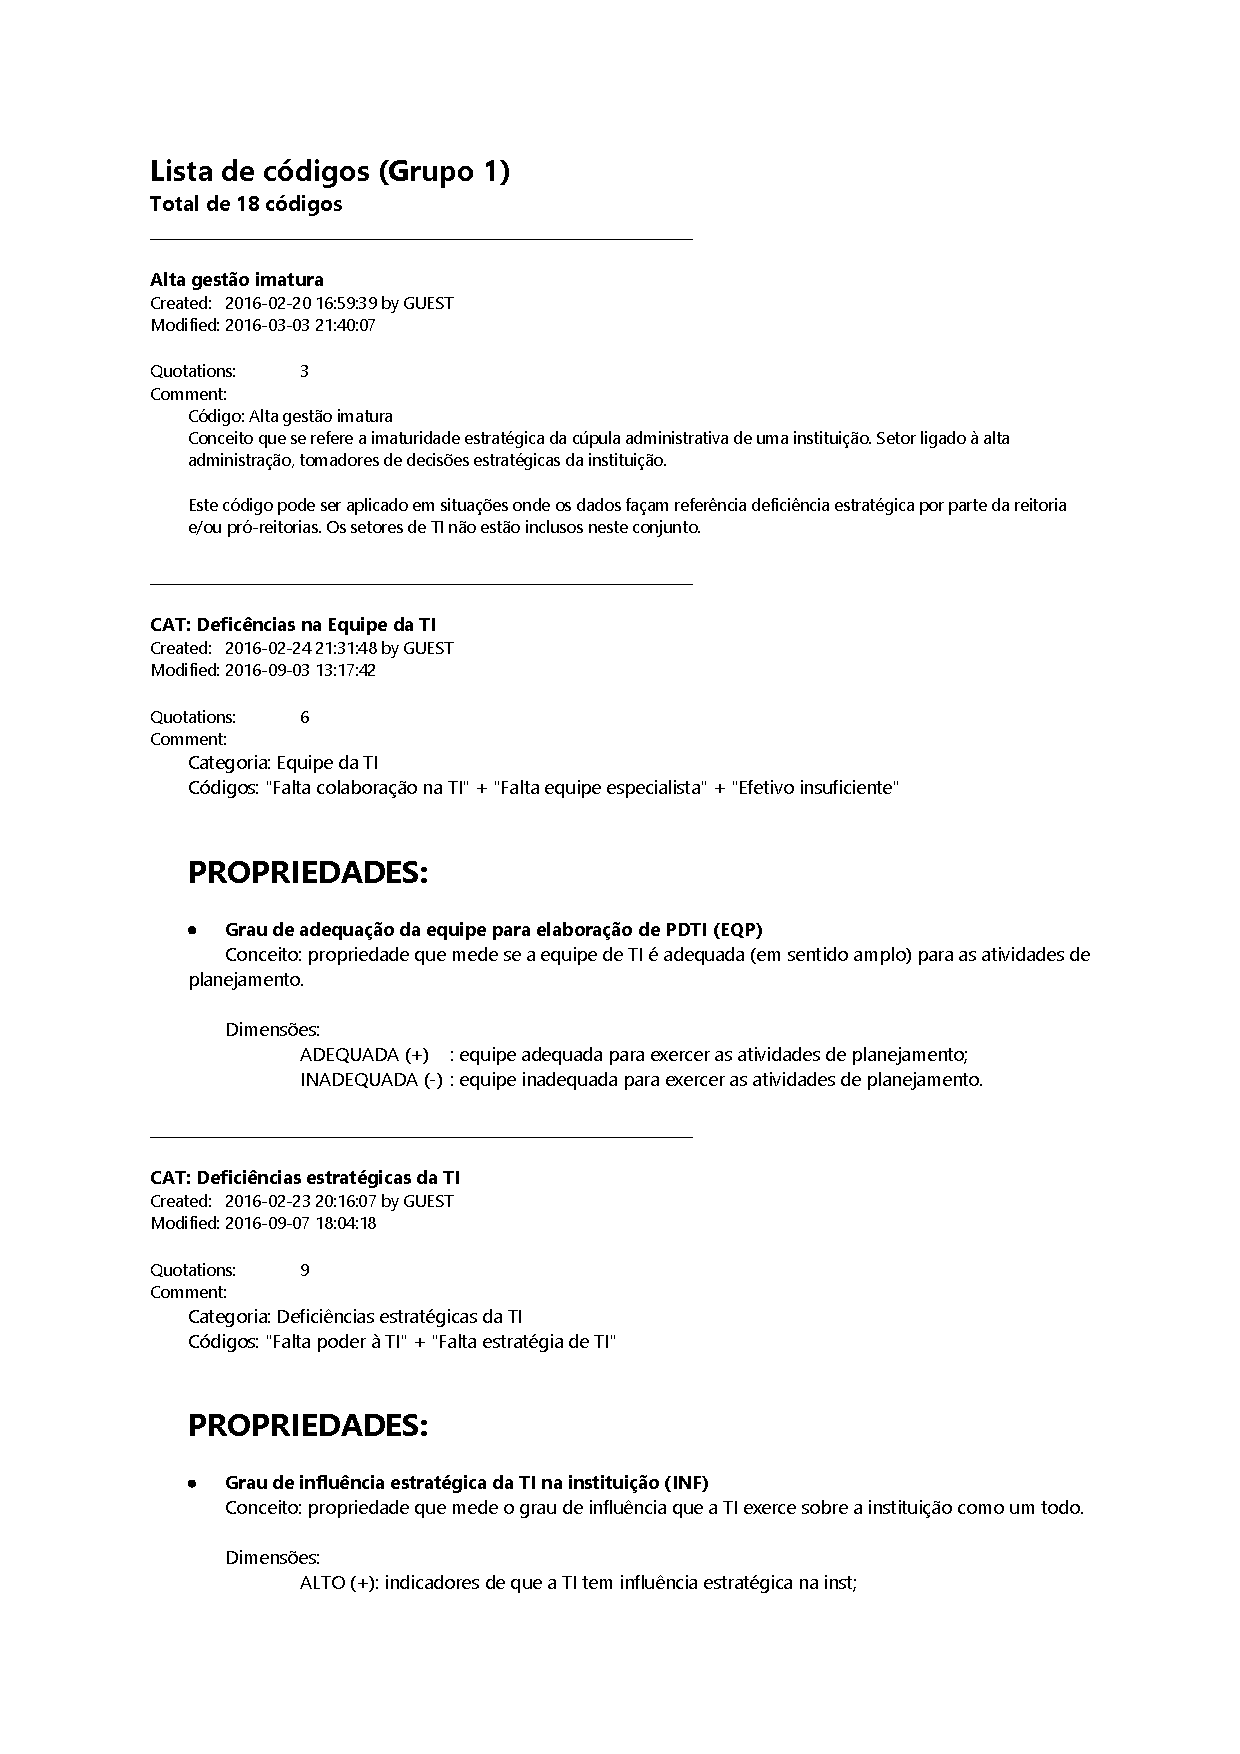
\includepdf[pages=-]{includes/apendiceE_codigos_g1.pdf}


\section{Citações por código do Grupo 1}
As páginas a seguir contém um relatório completo dos 18 códigos mapeados no grupo 1. O relatório apresenta cada citação vinculada a cada código, ou seja, cada trecho das respostas dos participantes que originou determinado código. Além disso, o relatório apresenta os códigos que possuem relacionamento entre si.

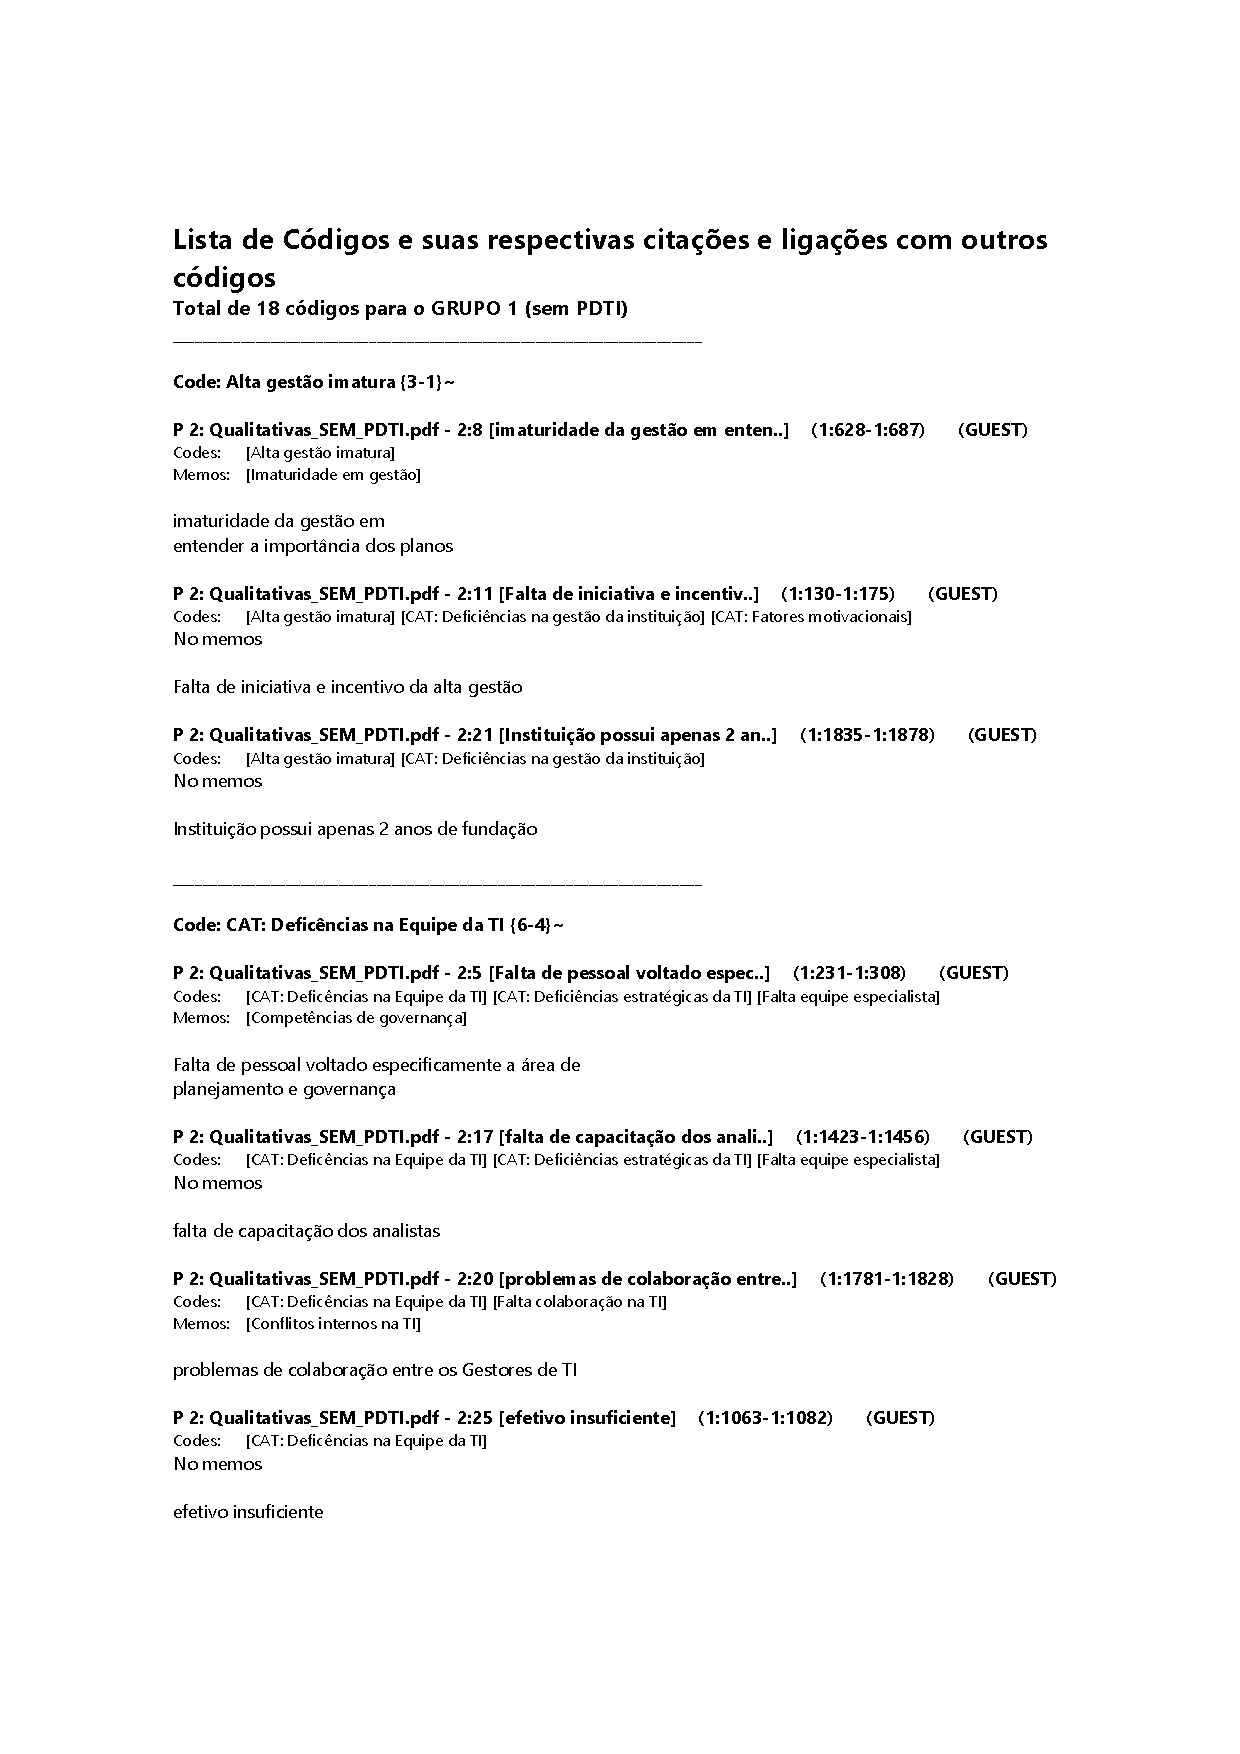
\includepdf[pages=-]{includes/apendiceE_codigos_e_citacoes_g1.pdf}


\section{Códigos do Grupo 2 (com PDTI)}
As páginas a seguir compõem o relatório de códigos mapeados no grupo 2. Totalizando 75 códigos, o relatório apresenta a definição de cada código, comentários, além de propriedades e dimensões dos códigos do tipo categoria.

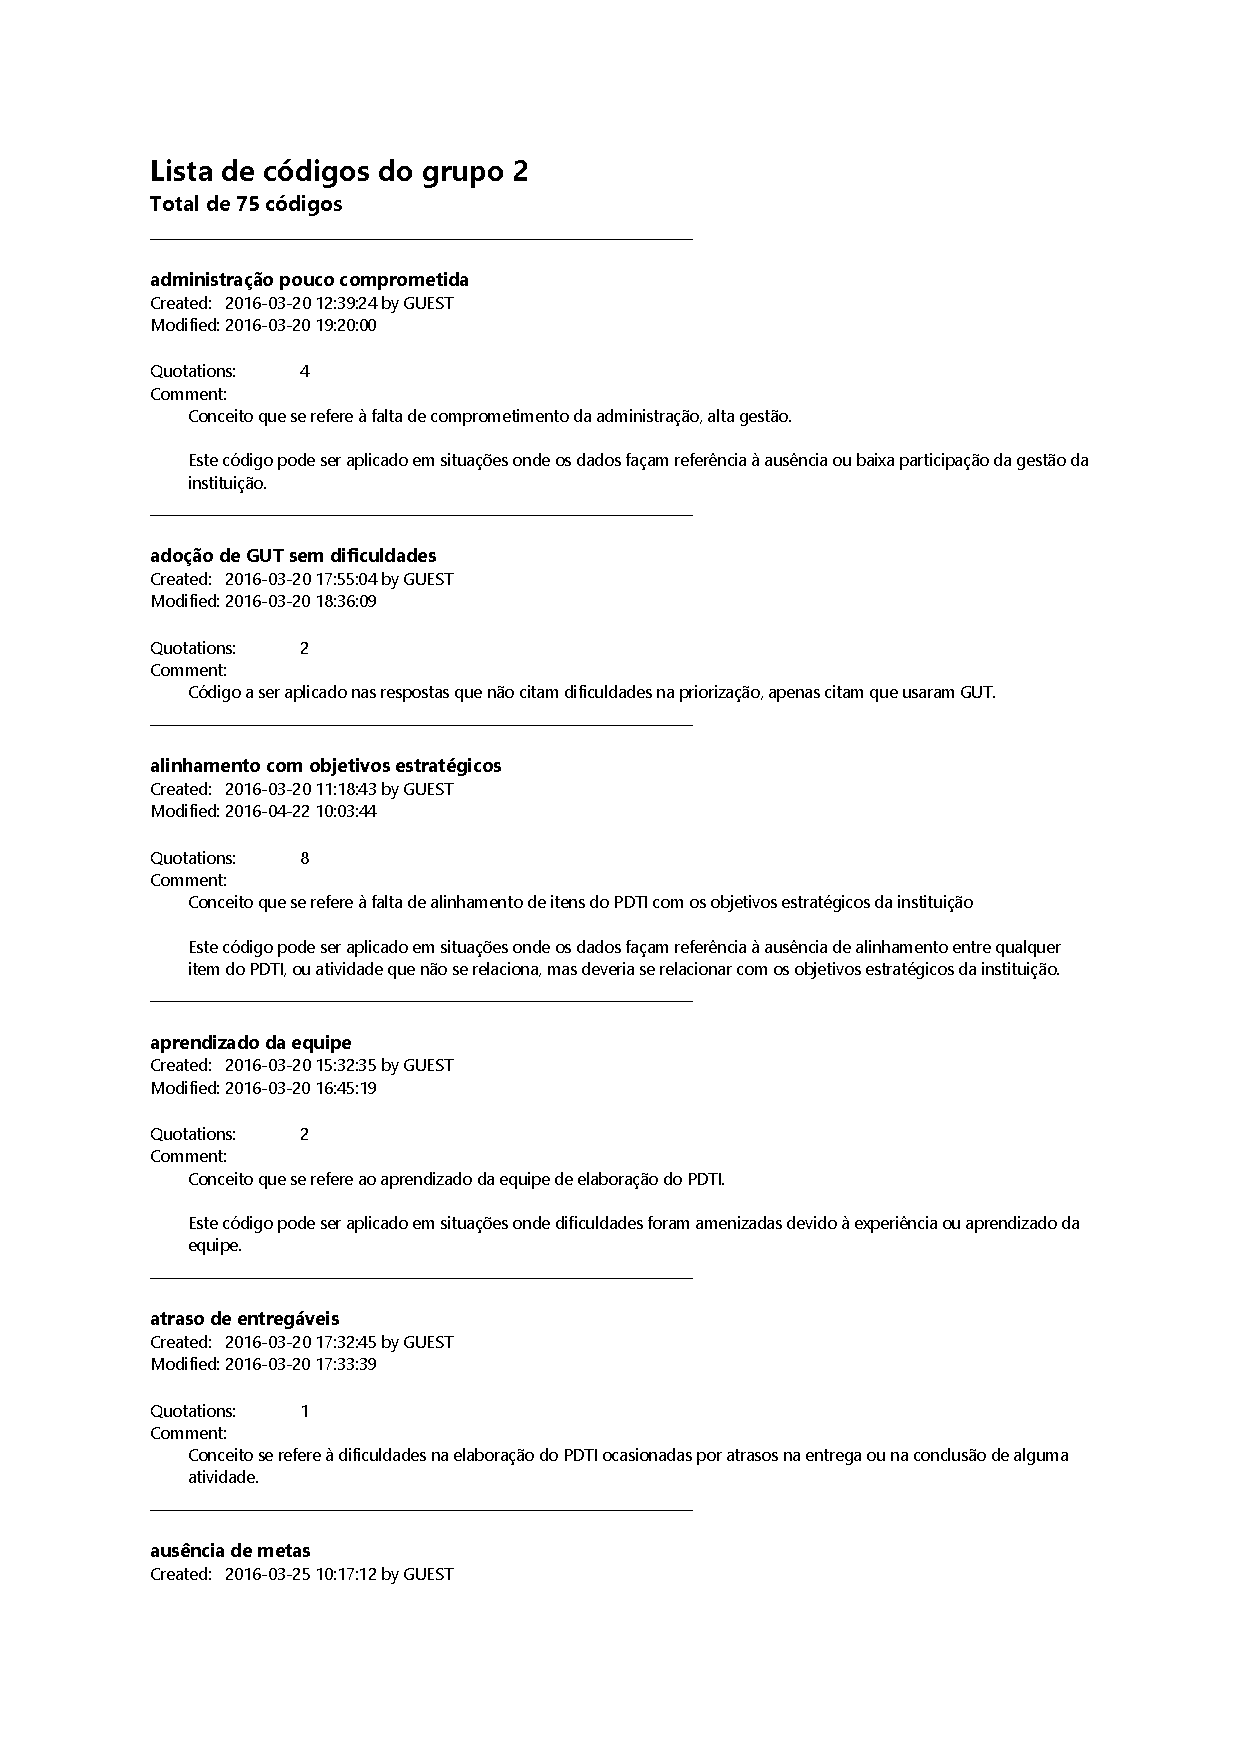
\includepdf[pages=-]{includes/apendiceE_codigos_g2.pdf}


\section{Citações por código do Grupo 2}
As páginas a seguir contém um relatório completo dos 75 códigos mapeados no grupo 2. O relatório apresenta cada citação vinculada a cada código, ou seja, cada trecho das respostas dos participantes que originou determinado código. Além disso, o relatório apresenta os códigos que possuem relacionamento entre si.

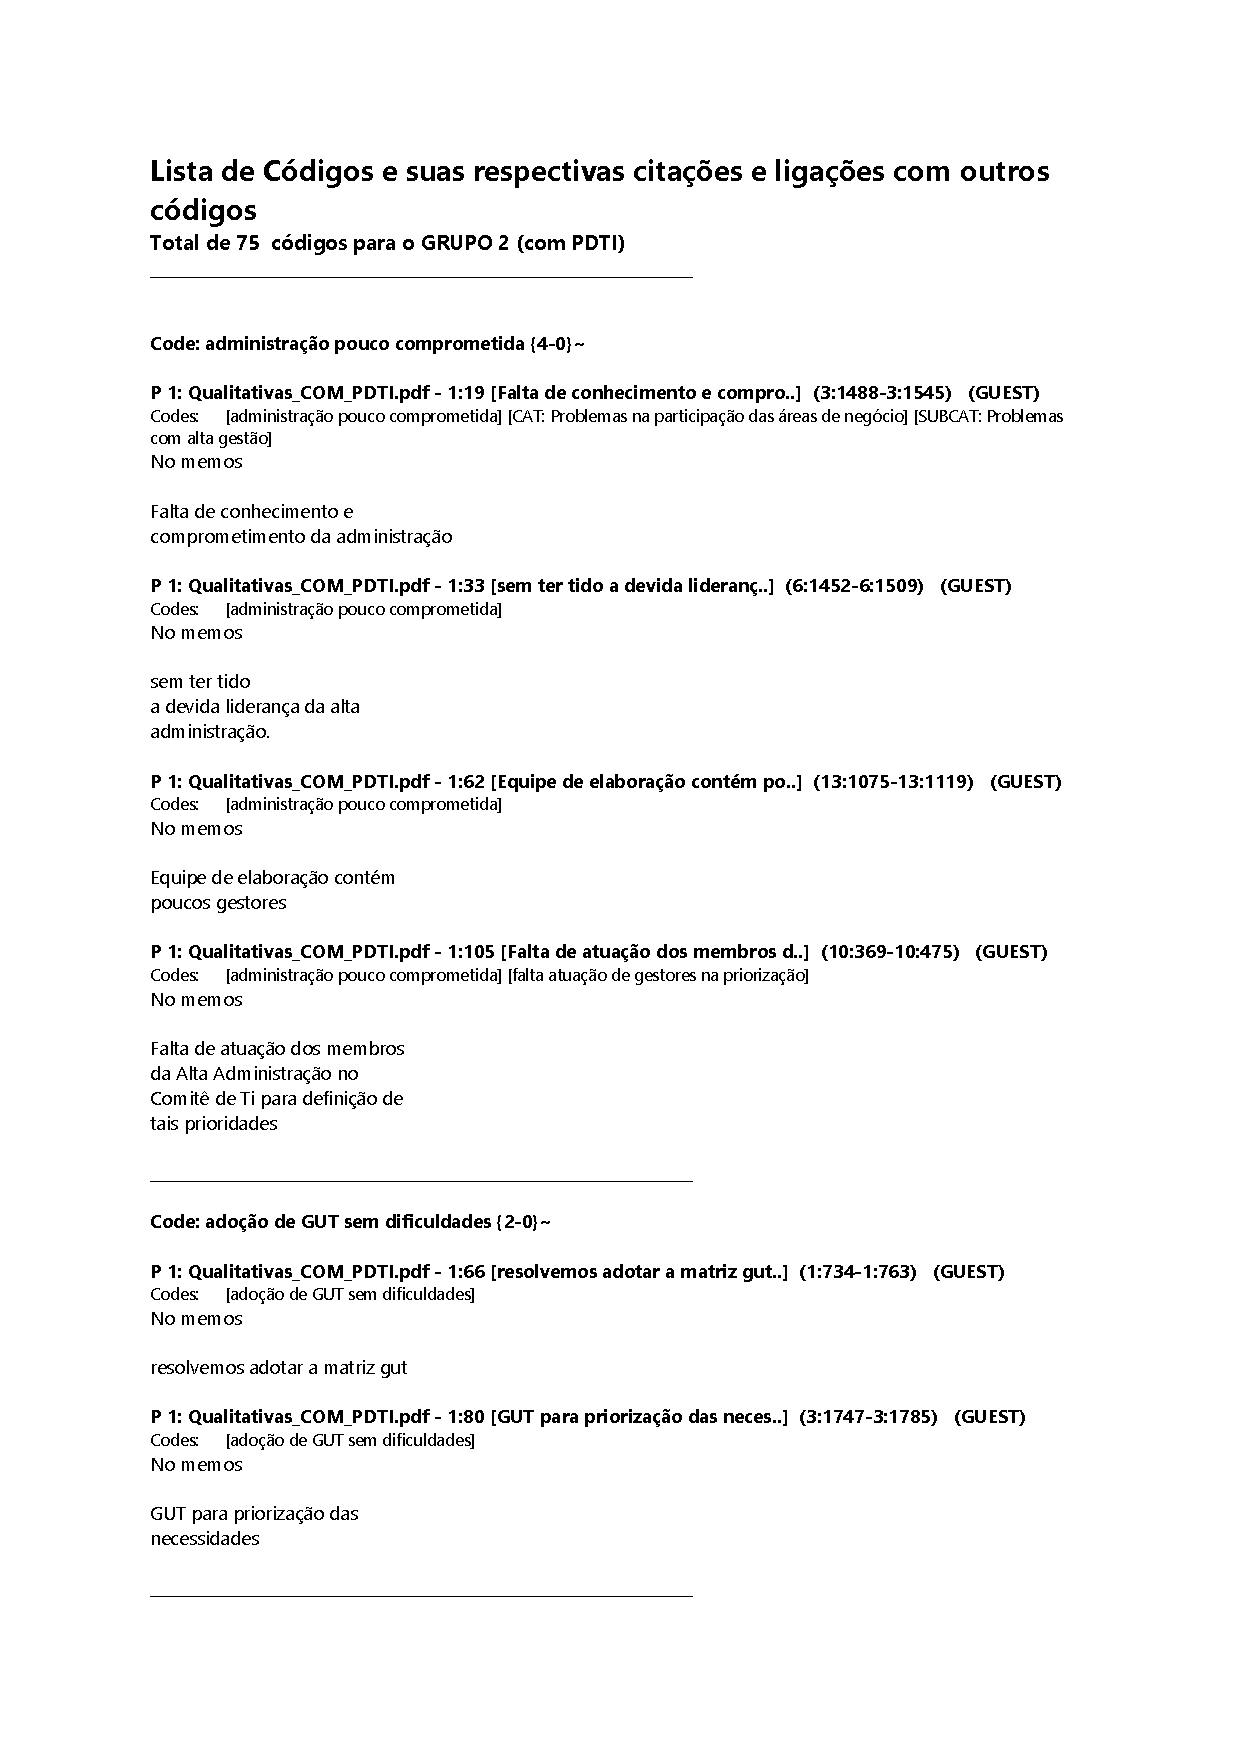
\includepdf[pages=-]{includes/apendiceE_codigos_e_citacoes_g2.pdf}